\documentclass[superscriptaddress, onecolumn, 11pt]{revtex4-1}
% preamble:

\usepackage{amsmath}    % need for subequations
\usepackage{graphicx}   % need for figures
\usepackage{verbatim}   % useful for program listings
\usepackage{color}      % use if color is used in text
\begin{comment}
\usepackage{subfigure}  % use for side-by-side figures
\end{comment}
\usepackage{hyperref}   % use for hypertext links, including those to external documents and URLs
\usepackage{amsmath,amssymb}
\raggedbottom           % don't add extra vertical space
\begin{comment}
\pagestyle{empty}       % use if page numbers not wanted
\end{comment}

\begin{document}

\title{
Sample \TeX file for paper writing
}

\author{K. Fujii}
\affiliation{
Department of Mechanical Engineering and Science, \\
Graduate School of Engineering, Kyoto University, \\
Kyoto 615-8540, Japan,\\
Email: fujii@me.kyoto-u.ac.jp}
\author{T. Kyodai}
\affiliation{
Some Institute, \\
Toki 123-4567, Japan}
}

\date{\today}

\begin{abstract}
  This is a sample file for the scientific paper writing.
\end{abstract}

\maketitle
\newcommand{\argmin}{\mathop{\mathrm{argmin}}\limits}
\newcommand{\bvec}[1]{\mathbf #1}


{\section{Introduction}
Introduction should be something like this.

In order to cite reference, do something like this,
\cite{Fujii2014}.

%--------------------------------------------------------------
\begin{figure*}[h!]
\centering
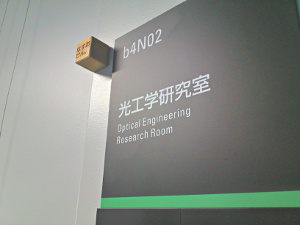
\includegraphics[scale=0.55]{figs/hikari_kogaku}
\caption{
\label{fig:TeNe}
Here is the figure caption.
}
\end{figure*}

%------------------------------------------------------



\section{Summary}
Here is the summary section.

\section*{Acknowledgement}
Acknowledgement should be coming here if necessary.

\bibliography{refs}

\end{document}
